\documentclass[tikz]{article}

% Packages
\usepackage[utf8]{inputenc} % Core latex bundle
\usepackage[a4paper, total={6in, 9in}]{geometry} % Customize document dimensions and formats
\usepackage{changepage} % Customize page layout in middle of document
\usepackage[table]{xcolor} % Add color to tables
\usepackage{standalone} % Add figures and tables from other files
\usepackage{import} % Import glossary
\usepackage{graphics} % General color and formats
\usepackage{url} % URL formatting
\usepackage{breakurl} % URL formatting
\usepackage{enumitem} % Format list spacing
\usepackage[hang]{footmisc} % Footnote margins
\usepackage{hyperref} % References
\usepackage{mathtools} % Useful tools for mathematical typesetting and replaces amsmath
\usepackage{amssymb,bm} % Math symbols
\usepackage{svg} % SVG
\usepackage{tikz} % Making charts
\usepackage{array,boldline,multirow,float,booktabs} % Added to make tables
\usepackage{stackengine} % Customize row heights
\usepackage{hhline} % Add double lines to table
\usepackage{multicol} % Two column lists
\usepackage{nicematrix} % Put table lines after color
\usepackage{wrapfig} % Wrap figures in text
\usepackage{tocloft,titletoc} % TOC package
\usepackage{titlesec} % Section spacing

% Paper formatting
\newlength\LabelWidth
\setlength\parindent{0pt}
\setlength{\parskip}{1em}

% Section spacing
\titlespacing*{\section}
{0pt}{0.6\baselineskip}{0.6\baselineskip} % Modify section spacing - first \baselineskip is spacing before, second is spacing after the section
\titlespacing*{\subsection}
{0pt}{0.6\baselineskip}{0.6\baselineskip} % Modify subsection spacing
\titlespacing*{\subsubsection}
{0pt}{0.6\baselineskip}{0.6\baselineskip} % Modify subsubsection spacing

% String formats
\newcommand{\code}[1]{\texttt{#1}}
\newcommand{\term}[1]{\textsl{#1}}

% Paper margins
\def\changemargin#1#2{\list{}{\rightmargin#2\leftmargin#1}\item[]}
\let\endchangemargin=\endlist

% Table of contents
\renewcommand{\contentsname}{Table of Contents}
\renewcommand{\cfttoctitlefont}{\Large\bfseries} % TOC title size
\renewcommand{\cftsecleader}{\cftdotfill{\cftdotsep}} % Add dots in TOC to sections
\renewcommand{\cftsecpagefont}{} % Remove \bfseries from section titles' page in TOC

% Section
\renewcommand*{\cftsecnumwidth}{2em} % Increase space section from numbers on left
% \setlength{\cftbeforesecskip}{3pt} % Messes with section TOC length

% Subsection
\cftsetindents{subsection}{1em}{3em} % space between numbers and toc subsections
\setlength{\cftsubsecindent}{2.5em} % subsection number spacing from left
\setlength{\cftbeforesubsecskip}{3pt} % Messes with subsection TOC length was 3pt

% Subsubsection
\cftsetindents{subsubsection}{1em}{4em} % space between numbers and toc subsubsections
\setlength{\cftsubsubsecindent}{5.5em} % subsubsection number spacing from leftindent
\setlength{\cftbeforesubsubsecskip}{3pt} % Messes with subsubsection TOC length was 3pt

% paragraph section
\setcounter{secnumdepth}{4}
\setcounter{tocdepth}{4}

\cftsetindents{paragraph}{1em}{5em} % space between numbers and toc paragraph
\setlength{\cftparaindent}{9.5em} % paragraph number spacing from leftindent
\setlength{\cftbeforeparaskip}{3pt} % Messes with paragraph TOC length was 3pt

% indent after paragraph section
\titleformat{\paragraph}
{\normalfont\normalsize\bfseries}{\theparagraph}{1em}{}
\titlespacing*{\paragraph}
{0pt}{3.25ex plus 1ex minus .2ex}{1.5ex plus .2ex}


% Abstract
% Make abstract justified
\makeatletter
\newcommand{\justified}{
\rightskip\z@skip
\leftskip\z@skip}
\makeatother

% Format and size abstract
\makeatletter
\renewenvironment{abstract}{
\if@twocolumn
\section*{\abstractname}
\else
\begin{center}
{\bfseries \large\abstractname\vspace{\z@}} % Bolds abstract name
\end{center}
\quotation
\fi}
{\if@twocolumn\else\endquotation\fi}
\makeatother

% Delimiters
\DeclarePairedDelimiter\floor{\lfloor}{\rfloor} % Define paired delimiter for floor function
\DeclarePairedDelimiter{\ceil}{\lceil}{\rceil} % Define paired delimiter for ceiling function

% Hyperlinks
\hypersetup{
colorlinks=true,
linkcolor=black,
filecolor=blue,
urlcolor=black,
}
\urlstyle{same}

% Footnotes
\newcommand{\fref}[1]{\footnote{\href{http://#1}{#1}}}
\setlength{\footnotemargin}{8mm} % Spacing between footnote number and body

% Include tables
\makeatletter
\newcommand{\includetable}[1]{%
\@ifundefined{tablepath}{%
\InputIfFileExists{#1}{}{}%
}{%
\InputIfFileExists{\tablepath/#1}{}{\InputIfFileExists{#1}{}{}}%
}
}
\makeatother

% Table formatting commands
\newcolumntype{Q}{ >{\centering\arraybackslash} m{2.4cm} } % (Figure 5 and 11 - col width)
\newcolumntype{S}{ >{\centering\arraybackslash} m{5.27cm} } % (Figure 12 - col width double)
\newcommand\xrowht[2][0]{\addstackgap[.5\dimexpr#2\relax]{\vphantom{#1}}} % Set row height for tables
\newcommand{\rowh}[1]{\xrowht{40pt}} % Command to set row height for cell with 3 rows
\newcommand{\rowm}[1]{\xrowht{26.667pt}} % Command to set row height for cell with 2 rows
\newcommand{\rows}[1]{\xrowht{13.333pt}} % Command to set row height for cell with 1 rows

% Bean symbols
\newcommand{\BeanCover}{\includesvg[scale=2.2]{./logos/black-bean.svg}} % Logo on cover page
\newcommand{\Bean}{\includesvg[scale=0.23]{./logos/bean.svg}} % Bean used throughout the paper in text form
\newcommand{\bean}{\includesvg[scale=0.17]{./logos/microbean-wide.svg}} % Bean used in formulas - micro bean wide
\newcommand{\tinybean}{\includesvg[scale=0.13]{./logos/microbean-wide.svg}} % Bean used in formulas - micro bean wide
\newcommand{\lambdabean}{\includesvg[scale=0.17]{./logos/microbean.svg}} % Bean used in formulas for lambda superscript - micro bean

% Pump symbols

\newcommand{\PumpCover}{\includesvg[scale=0.25]{./logos/multi-flow.svg}} % Logo on cover page

% List Key
\SetEnumitemKey{midsep}{topsep=0pt, itemsep=3pt} % Itemize key

% File paths
\newcommand{\tablepath}{figures} % Tables file path
\graphicspath{{figures/}} % Figures file path

%%%%%%% Begin Document %%%%%%%
\begin{document}
\pagenumbering{arabic} % Start page numbering style
\thispagestyle{empty} % Hide page numbering
\begin{titlepage}
\begin{center}
\vspace*{-0.1cm}
\begin{changemargin}{-1.5cm}{-1.5cm}
\centering % added to center title
\textbf{\Large{Multi Flow: Multi-block MEV Resistant Pump For Current Values}}
\end{changemargin}
\begin{center}
\PumpCover
\end{center}
\vspace{0.4cm}
\large{Publius}

\vspace{-0.25cm}
\normalsize{beanstalk.publius@protonmail.com}

\vspace{-0.25cm}
\normalsize{\href{https://basin.exchange/}{basin.exchange}}

\vspace{0.4cm}
\footnotesize{Published:} \normalsize{July UPDATE, 2023}

\vspace{-0.25cm}
\footnotesize{Modified:} \normalsize{July UPDATE, 2023}

\vspace{-0.25cm}
\footnotesize{Whitepaper Version:} {\normalsize{1.0.0}}

\vspace{-0.25cm}
\footnotesize{Code Version:} \href{https://github.com/BeanstalkFarms/Basin/blob/master/src/pumps/MultiFlowPump.sol}{\normalsize{1.0.0}}\footnote{\href{https://github.com/BeanstalkFarms/Basin/blob/master/src/pumps/MultiFlowPump.sol}{github.com/BeanstalkFarms/Basin/blob/master/src/pumps/MultiFlowPump.sol}}


\vspace{0.1cm}
\flushleft{\normalsize{\term{“So we sailed on through the narrow straits, crying aloud for fear of Scylla on the one hand while divine Charybdis sucked the sea in terribly on the other.”}}}

\normalsize{\hspace{2.5em}- Homer, The Odyssey}\fref{poetryintranslation.com/PITBR/Greek/Odyssey12.php}
\vspace{0.4cm}
\begin{abstract}
\justified{\normalsize{\noindent Oracles are a core piece of the decentralized financial tech stack. Non-network-native oracles that require additional trust assumptions beyond the integrity of the network are the only current option for EVM-native protocols in a post-Merge\fref{ethereum.org/en/roadmap/merge} environment because current network-native oracles are not resistant to multi-block maximum extractable value (MEV) manipulation. We propose a multi-block MEV resistant network-native oracle for arbitrary current data in an EVM for both instantaneous and time-weighted values.}}
\end{abstract}
\end{center}
\end{titlepage}

\newpage

% TOC formatting
% \addtocontents{toc}{\protect\enlargethispage{20mm}} % TOC margins
\thispagestyle{empty} % Hide TOC page numbering
\addtocontents{toc}{\protect\thispagestyle{empty}} % Allow hiding both TOC page numbers

\cleardoublepage
\pagenumbering{gobble}
{\large\tableofcontents} % Compile TOC with large font
\cleardoublepage
\pagenumbering{arabic}

% \thispagestyle{empty} % Hide TOC page numbering
% \addtocontents{toc}{\protect\thispagestyle{empty}} % Allow hiding both TOC page numbers

\newpage
\setcounter{page}{3} % Begin page numbering

\section{Introduction}
Oracles are the basis for any complex network-native financial activity: network-native contracts often require oracles to report data external to it to process transactions. Oracle data can be bifurcated into data that is native to the network of the contracts using the oracle data and data that is not native to the network. Whereas data that is not native to the network must be reported to the network through some external oracle system that requires additional trust assumptions beyond the integrity of the network itself, data that is native to the network can be reported through a network-native oracle that does not. However, there are no current Ethereum-native oracles for Ethereum-native data that offer manipulation resistance in a post-Merge environment. 

Prior to the Merge the potential for “risk-free” manipulation resistance was limited to intra-block (\textit{i.e.}, within a single block) manipulation. However, the Merge created the potential for “risk-free” inter-block (\textit{i.e.}, across multiple blocks) manipulation because block proposers are known at the beginning of each epoch. When the same proposer (or a coordinated set of proposers) know they get to propose multiple consecutive blocks, they can execute arbitrary activity acceptable to the network (\textit{e.g.}, buy as much of an asset as possible) without risk of having any transactions processed that cost them anything (\textit{e.g.}, selling the asset at its now elevated price) until the first block they are not the proposer of. All oracles for network-native data that were implemented prior to the Merge lack inter-block manipulation resistance. The occurence of consecutive blocks being proposed by the same proposer is high enough\fref{alrevuelta.github.io/posts/ethereum-mev-multiblock} such that current network-native oracles are unusable for any protocol that requires manipulation resistant oracles. 

%\vspace*{-3mm}
\begin{figure}[h!]
    \centering
    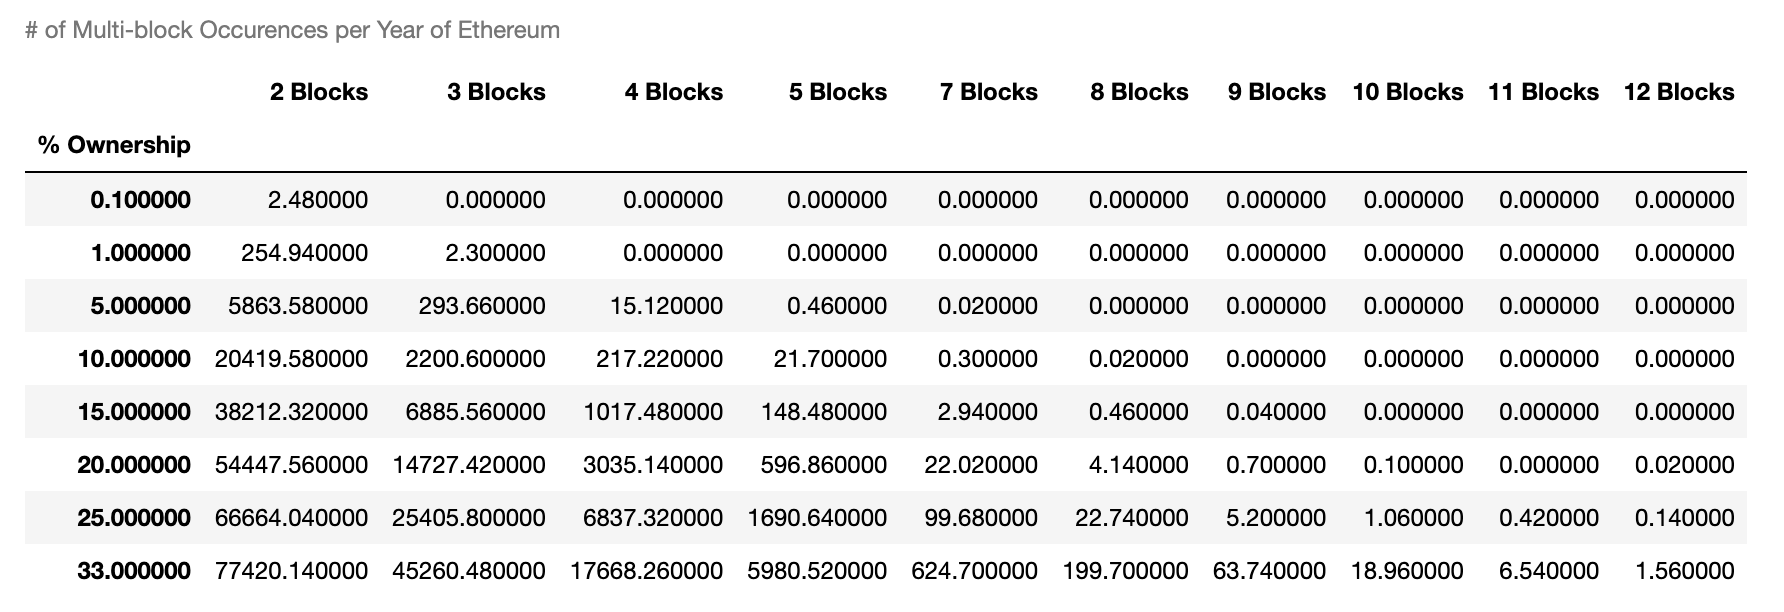
\includegraphics[scale=.25]{Figure15}
    \vspace*{-5mm}
    \caption{Multi-Block MEV Occurences Per Year By Validator Ownership Percent}
    \label{fig 2}
\end{figure}
%\vspace*{-5mm}

Basin is a composable decentralized exchange (DEX) architecture native to the EVM(UPDATE CITE BASIN WP). Pumps are the generalized oracle component of Basin. The ability to compose together arbitrary exchange functions and oracles with Basin allows for the combination of existing exchange functions that remain popular for network-native exchanges with new network-native oracles that are multi-block MEV manipulation resistant.

Oracle data can be further classified as current or historical data, and instantaneous or time-weighted. Whereas there is inherently no network-native oracle for non-network-native data, there are potential network-native oracles for current and historical data of instantaneous and time-weighted values. Multi Flow supports current instantaneous and time-weighted values to allow for any network-native protocol to access manipulation resistant current data stored in a Multi Flow from a network-native oracle.

\section{Previous Work}
Multi Flow is the next step in the evolution of EVM-native oracles for current values.

A robust, trustless computer network that supports composability and fungible token standards (\textit{i.e.}, Ethereum) is necessary to host a DEX. A DEX that supports the composition of other components of an exchange with arbitrary oracles (\textit{i.e.}, Basin) and an interface for arbitrary oracles (\textit{i.e.}, \term{Pumps}) is necessary to support Multi Flow. 

Uniswap V2\fref{uniswap.org/whitepaper.pdf} implemented a time-weighted average (TWA) network-native oracle for assets being traded in a Uniswap V2 liquidity pool by saving a cumulative sum of the time-weighted prices of the pool at the end of the last block a trade occurred in. Using the end of block price prevented intra-block manipilation but does not provide any inter-block manipulation resistance. Uniswap V2 does not store historical cumulative values of the oracle, such that other protocols wishing to use the oracle must store historical values as necessary. The Uniswap V2 oracle lacks support for an inter or intra-block manipulation resistant current price. 

Curve\fref{etherscan.io/token/0xc9c32cd16bf7efb85ff14e0c8603cc90f6f2ee49} impelemented an intra-block manipulation resistant current price oracle using the price at the end of the last block. The Curve oracle lacks support for an inter-block manipulation resistant current price. 

Uniswap V3\fref{uniswap.org/whitepaper-v3.pdf} innovated further on manipulation resistant network-native oracles for time-weighted values by moving from a simple moving average (SMA) of an arithmetic mean,\fref{uniswap.org/whitepaper.pdf} which weights outliers equally to all other data points, to an SMA of a geometric mean, which weights certain outliers significantly less. In addition to price, the oracle also stores data related to the liquidity in the pool, such that time and liquidity-weighted prices can be computed. The V3 oracle stores historical oracle values making it unnecessary for other protocols to do so. 

\section{Multi Flow}
Multi Flow takes a two-step approach to creating a network-native multi-block MEV manipulation resistant oracle from manipulable data. First, Multi Flow “cleans” the data by calculating multi-block MEV manipulation resistant last values. Then, using the manipulation resistant last values, Multi Flow calculates current instantaneous and time-weighted multi-block MEV manipulation resistant values. 

In practice Multi Flow stores 3 different types of values at the last updated timestamp ($l$), such that $l, x \in \mathbb{Z}^{+}$:
\begin{itemize}
\item Multi-block MEV resistant last values: $[x^{MEV}_{0,l}, \cdots, x^{MEV}_{n,l}]$,
\item Multi-block MEV resistant Geometric EMA values: $[x^{EMA}_{0,l}, \cdots, x^{EMA}_{n,l}]$, and
\item Multi-block MEV-resistant Cumulative Geometric SMA values: $[x^{SMA}_{0,l}, \cdots, x^{SMA}_{n,l}]$.
\end{itemize}

All values are stored in $log_2$ form. To properly read each value from Multi Flow, they must be converted to their normal form. Therefore, Multi Flow supports 3 different types of values at timestamp $t$, such that $l \leq t$, $t, y \in \mathbb{Z}^{+}$:
\begin{itemize}
\item Multi-block MEV resistant last values: $[y^{MEV}_{0,l}, \cdots, y^{MEV}_{n,l}]$,
\item Multi-block MEV resistant Geometric EMA values: $[y^{EMA}_{0,l}, \cdots, y^{EMA}_{n,l}]$, and
\item Multi-block MEV-resistant Cumulative Geometric SMA values: $[y^{SMA}_{0,t_0,t_1}, \cdots, y^{SMA}_{n,t_0,t_1}]$.
\end{itemize}

In addition to reading the values stored at timestamp $l$, Multi Flow also supports reading the current values at timestamp $t$.

\subsection{Multi-Block MEV Manipulation Resistant Last Values}
In a post-Merge multi-block MEV susceptible environment there is no way for network-native oracles to know whether the data at the beginning or end of a particular transaction or block is being manipulated or not. In practice this means that oracles must assume the potential for manipulation of every value. Therefore, the fundamental question for manipulation resistant oracles in a multi-block MEV enviroment is around the treatment of statistical outliers which are certain to exist with no way for the oracle to know if it is the result of honest network activity or manipulation. 

The multi-block MEV manipulation resistant last values are calculated using a cap on the maximum percent change of the values acceptable per block. The cap limits the extent of manipulation over a given period of time and in doing so “cleans” the data for postprocessing into current instantaneous and time-weighted oracle values. 

For a given maximum increase permitted of a value per block ($\gamma_+$), maximum decrease permitted of a value per block ($\gamma_-$), block time of the given EVM in seconds ($\beta$), such that $\gamma_+,\ \gamma_-,\ \beta, \in \mathbb{Z}^{+}$, and the current values ($[x_{0,t}, \cdots, x_{n,t}]$), Multi Flow updates $[x^{MEV}_{0,l}, \cdots, x^{MEV}_{n,l}]$ at timestamp $t$ as:
$$
x^{MEV}_{i,t} = 
\begin{cases}
min\left(x_{i,t}, x^{MEV}_{i,l}(1+\gamma_+)^\frac{t-l}{\beta}\right) & x_{i,t} > x^{MEV}_{i,l} \\
max\left(x_{i,t}, x^{MEV}_{i,l}(1-\gamma_-)^\frac{t-l}{\beta}\right) & \text{otherwise} \\
\end{cases}
$$

Because exponentiation is expensive in the EVM, in practice $[x^{MEV}_{0,l}, \cdots, x^{MEV}_{n,l}]$ is updated at $t$ as:
$$
x^{MEV}_{i,t} = 
\begin{cases}
min\left(log_2(x_{i,t}), x^{MEV}_{i,l} + log_2(1+\gamma_+) \frac{t-l}{\beta}\right) & log_2(x_{i,t}) > x^{MEV}_{i,l} \\
max\left(log_2(x_{i,t}), x^{MEV}_{i,l} + log_2(1-\gamma_-) \frac{t-l}{\beta}\right) & \text{otherwise} \\
\end{cases}
$$

Therefore, the mutli-block MEV manipulation resistant last values can be read as: 
$$
y^{MEV}_{i,l} = 2^{x^{MEV}_{i,l}}
$$

\subsection{Multi-Block MEV Manipulation Resistant Instantaneous Values}
Multi Flow uses an exponential moving average (EMA) of the multi-block MEV resistant last values to calculate multi-block MEV manipulation resistant current instantaneous values. EMAs are useful for aggregating a time-series of data into a single value and are preferable to SMAs for instantaneous value because (1) they weight recent data more than older data and (2) instances where the direction in the deviations of the new last value and EMA value from the old ones are different are much more limited in frequency and scale (\textit{i.e.}, their changes are directionally the same more often). An EMA of the multi-block MEV resistant last values is preferable to the multi-block MEV resistant last values for reading an instantaneous value because it requires manipulation over extended periods of time to significantly manipulate the value.

For a given exponential decay parameter ($\alpha$), such that $\alpha \in (0,1)$, $[x^{EMA}_{0,l}, \cdots, x^{EMA}_{n,l}]$ and $[x^{MEV}_{0,t}, \cdots, x^{MEV}_{n,t}]$, Multi Flow updates $[x^{EMA}_{0,t}, \cdots, x^{EMA}_{n,t}]$ at timestamp $t$ as:
$$
x^{EMA}_{i,t} = \alpha^{t-l} x^{EMA}_{i,l} + (1 - \alpha^{t-l}) x^{MEV}_{i,t}
$$

Therefore, the multi-block MEV manipulation resistant current instantaneous values can be read as: 
$$
y^{EMA}_{i,l} = 2^{x^{EMA}_{i,l}}
$$

\subsection{Multi-Block MEV-Resistant Time-Weighted Average Values}
Multi Flow uses a cumulative sum of the multi-block MEV resistant last values to calculate multi-block MEV resistant SMA values. SMAs are useful for aggregating a time-series of data into a single value and are preferable to EMAs for time-weighted average value because they weight recent data the same as older data.

For a given $[x^{SMA}_{0,l}, \cdots, x^{SMA}_{n,l}]$ and $[x^{MEV}_{0,t}, \cdots, x^{MEV}_{n,t}]$, Multi Flow updates $[x^{SMA}_{0,t}, \cdots, x^{SMA}_{n,t}]$ at timestamp $t$ as:
$$
x^{SMA}_{i,t} = x^{SMA}_{i,l} + (t-l) x^{MEV}_{i,t}
$$

Therefore, the multi-block MEV manipulation resistant TWA values can be calculated from $x^{SMA}_{i,t_0}$ and $x^{SMA}_{i,t_1}$ as:
$$
y^{SMA}_{i,t_0,t_1} = 2^{\frac{x^{SMA}_{i,t_1} - x^{SMA}_{i,l}}{t_1-t_0}}
$$

Because only the latest values of $[x^{SMA}_{0,t}, \cdots, x^{SMA}_{n,t}]$ are stored by Multi Flow, protocols must snapshot values at the beginning of the period over which the time-weighted average is being measured.

\subsection{Governance}
Multi Flow is non-upgradable. Therefore, there Multi Flow does not support governance.

\section{Risks}
There are numerous risks associated with Multi Flow. This is not an exhaustive list.

The Multi Flow code base is novel. It has not been tested in the “real world” prior to its initial deployment. The open source nature of Multi Flow means that others can take advantage of any bugs, flaws or deficiencies in it. While Multi Flow has been audited(UPDATE AUDIT LINK) it is no guarantee of security. 

The Multi Flow does not prevent the manipulation of network-native values. Instead, it minimizes the effect of manipulation on oracle values(UPDATE). Therefore Multi Flow is manipulation resistant, not manipulation-preventing. 

\section{Future Work}
Manipulation resistant network-native oracles are a work in progress. The following are potential improvements that can be incorporated into future iterations of manipulation resistant network-native oracles:

\begin{itemize}
\item Support for historical values.
\item Support for additional data (\textit{e.g.}, volatility).
\item The ability to turn off when manipulation is detected.
\item The ability to reset if it breaks.
\end{itemize}

\end{document}
